\chapter{三角比与角边关系}

人们为了要确定空间各点之间的相互位置,就得做一番
测量,测量是几何学的起源,也是几何学最直接的实践。

测量学的最基本原理,就是相似形的性质及三角形的边
角关系。例如,我们在第三章末用相似形性质测量两点间的,
距离,物体的高度、测绘具有多边形形状的地段的平面图
等。我们知道,在两个直角三角形中,只要有一个锐角对应
相等,它们就相似了,这就是说,一个直角三角形的各边之。
间的比是被它的一个锐角的大小所决定,例如在图6.1中,
一些含有$30^{\circ}$角的直角三角形,$30^{\circ}$角所对的直角边与斜边的
比都是1:2.

\begin{figure}[htp]
    \centering
\begin{tikzpicture}
\begin{scope}
\tkzDefPoint(30:2){B_1}
\tkzDefPoints{0/0/A_1, 1.732/0/C_1}
\tkzDrawPolygon(A_1,B_1,C_1)
\tkzMarkAngle[mark=none, size=.5](C_1,A_1,B_1)
\tkzLabelPoints[right](C_1,B_1)
\tkzLabelPoints[left](A_1)
\tkzMarkRightAngle(B_1,C_1,A_1)
\end{scope}
\begin{scope}[xshift=3.5cm]
    \tkzDefPoint(30:3){B_2}
    \tkzDefPoints{0/0/A_2, 2.6/0/C_2}
    \tkzDrawPolygon(A_2,B_2,C_2)
    \tkzMarkAngle[mark=none, size=.5](C_2,A_2,B_2)
    \tkzLabelPoints[right](C_2,B_2)
    \tkzLabelPoints[left](A_2)
    \tkzMarkRightAngle(B_2,C_2,A_2)
\end{scope}
\begin{scope}[xshift=11cm]
    \tkzDefPoint(150:4){B_3}
    \tkzDefPoints{0/0/A_3, -3.464/0/C_3}
    \tkzDrawPolygon(A_3,B_3,C_3)
    \tkzMarkAngle[mark=none, size=.6](B_3,A_3,C_3)
    \tkzLabelPoints[below](C_3,A_3)
    \tkzLabelPoints[left](B_3) 
    \tkzMarkRightAngle(A_3,C_3,B_3)
\end{scope}

\end{tikzpicture}
    \caption{}
\end{figure}

这一章,我们首先向同学介绍的就是直角三角形中,边
与边的比与它所含锐角之间的关系。这些边与边的比值叫做
\textbf{锐角三角比},它们是进行测量计算时的常用数据,也是从数
量方面研究几何学的基本工具。

\section{锐角三角比}

\subsection{定义}

\begin{figure}[htp]\centering
    \begin{minipage}[t]{0.48\textwidth}
    \centering
\begin{tikzpicture}[>=latex, scale=.8]
\draw(30:6)node[right]{$Y$}--(0,0)node[left]{$A$}--(5.5,0)node[right]{$X$};
\draw(30:5)node[above]{$B$}--node[right]{$a$}+(0,-2.5)node[below]{$C$};
\node at (1.25*1.732,0)[below]{$b$};
\node at (30:2.5)[above]{$c$};
\draw(4.33,0) rectangle (4.33-.2,.2);
    \end{tikzpicture}
    \caption{}
    \end{minipage}
    \begin{minipage}[t]{0.48\textwidth}
    \centering
    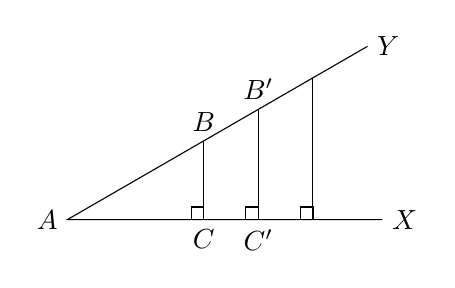
\begin{tikzpicture}[>=latex, scale=.8]
\draw(30:5.5)node[right]{$Y$}--(0,0)node[left]{$A$}--(5,0)node[right]{$X$};
\draw(30:2.5)node[above]{$B$}--+(0,-1.25)node[below]{$C$};
\draw(30:3.5)node[above]{$B'$}--+(0,-1.75)node[below]{$C'$};
\draw(30:4.5)--+(0,-2.25);
\draw(2.165,0) rectangle (2.165-.2,.2);
\draw(3.03,0) rectangle (3.03-.2,.2);
\draw(3.9,0) rectangle (3.9-.2,.2);
    \end{tikzpicture}
    \caption{}
    \end{minipage}
    \end{figure}


取任意锐角$\angle XAY$, 在边$AY$上任取一点$B$, 作$\overline{BC}\bot AX$
于$C$(图6.2). 在直角$\triangle ABC$中,设$\angle A$、$\angle B$、$\angle C$的
对边分别用$a$、$b$、$c$表示,对
锐角$A$来说,$a$叫做$\angle A$的\textbf{对
边},$b$叫做$\angle A$的相邻的直角
边(简称\textbf{邻边})我们定义:
\begin{enumerate}
    \item $\angle A$的对边与斜边的比值,叫做$\angle A$的正弦,用符
号$\sin A$来表示,即
\[\sin A=\frac{\angle A\text{的对边}}{\text{斜边}}=\frac{a}{c}\]
\item $\angle A$的邻边与斜边的比值,叫做$\angle A$的余弦。用符
号$\cos A$来表示,即
\[\cos A=\frac{\angle A\text{的邻边}}{\text{斜边}}=\frac{b}{c}\]
\item $\angle A$的对边与邻边的比值,叫做$\angle A$的正切,用符
号$\tan A$来表示,即
\[\tan A=\frac{\angle A\text{的对边}}{\angle A\text{的邻边}}=\frac{a}{b}\]
\item $\angle A$的邻边与对边的比值,叫做 $\angle A$的余切,用符
号$\cot A$来表示,即
\[\cot A=\frac{\angle A\text{的邻边}}{\angle A\text{的对边}}=\frac{b}{a}\]
\end{enumerate}

我们知道,只要$\angle A$的大
小定了,不管$B$点在边$AY$上
的位置如何(图6.3),以上
的四个比值都是不变的,只有
当$\angle A$变化时,这些比值才随着变化。这四个比都叫做锐角$A$的三角比。

有了以上定义,我们就在直角三角形的角与边之间建立
了联系,知道了角的大小,相应的四个三角比就被唯一地确
定了。反过来,如果我们知道了一个角的四个三角比中的任
何一个,我们也就能确定这个角的大小。

\begin{example}
    在直角$\triangle ABC$中,$\angle C=90^{\circ}$, $\overline{BC}=3$cm, $\overline{AC}=
    4$cm, 求$\angle A$的4个三角比(图6.4)。
\end{example}

\begin{figure}[htp]\centering
    \begin{minipage}[t]{0.48\textwidth}
    \centering
\begin{tikzpicture}[>=latex, scale=1]
\draw(0,0)node[left]{$B$}--node[below]{3}(3,0)node[right]{$C$}--node[right]{4}(3,4)node[above]{$A$}--node[left]{5}(0,0); 
\draw(3,0) rectangle (3-.2,.2);
\draw(3,4-.5) arc (-90:-36.9-90:.5);

    \end{tikzpicture}
    \caption{}
    \end{minipage}
    \begin{minipage}[t]{0.48\textwidth}
    \centering
    \begin{tikzpicture}[>=latex, scale=.8]
\draw(40:7)node[right]{$Y$}--(0,0)node[left]{$A$}--(5,0)node[right]{$X$};
\draw(4.2,0)node[below]{$C$}--node[right]{$1.8$}(4.2,3.56)node[above]{$B$};
\node at (40:3)[left]{$3$};
\node at (2.1,0)[below]{$2.1$};
\draw(4.2,0) rectangle (4,.2);
\draw(.5,0) arc (0:40:.5);
    \end{tikzpicture}
    \caption{}
    \end{minipage}
    \end{figure}

\begin{solution}
    根据勾股定理,
  \[  \overline{AB}=\sqrt{\overline{BC}^2+\overline{AC}^2}=\sqrt{3^2+4^2}=5{\rm (cm)}\]
  根据各三角比的定义有,
\[\begin{split}
    \sin A=\frac{\overline{BC}}{\overline{AB}}=\frac{3}{5},&\qquad \cos A=\frac{\overline{AC}}{\overline{AB}}=\frac{4}{5}\\
    \tan A=\frac{\overline{BC}}{\overline{AC}}=\frac{3}{4},&\qquad \cot A=\frac{\overline{AC}}{\overline{BC}}=\frac{4}{3}\\
\end{split}\]
\end{solution}


\begin{example}
      求$40^{\circ}$角的四个三角比。
\end{example}

\begin{solution}
 用量角器画$\angle XAY=40^{\circ}$(图6.5). 在边$AY$上截
取$\overline{AB}=3$cm(为计算方便,我们尽量取整数),作$\overline{BC}\bot AY$于$C$点,量得$\overline{BC}=1.8$cm, $\overline{AC}=2.1$cm, 在直角
$\triangle ABC$中,根据三角比的定义可得:
\[\sin40^{\circ}=\frac{1.8}{3}\approx 0.6,\qquad \cos40^{\circ}=\frac{2.1}{3}\approx 0.7 \]
\[\tan40^{\circ}=\frac{1.8}{2.1}\approx 0.8,\qquad \cot40^{\circ}=\frac{2.1}{1.8}\approx 1.1\]
\end{solution}

\begin{example}
    已知$\tan A=\frac{1}{2}$, 求$\angle A$.
\end{example}

\begin{figure}[htp]
    \centering
\begin{tikzpicture}
\draw(0,0)node[left]{$A$}--(4,0)node[right]{$C$}--(4,2)node[above]{$B$}--(0,0);
\draw (4,0)rectangle(4-.2,.2);
\end{tikzpicture}
    \caption{}
\end{figure}

\begin{solution}
    作一个直角$\triangle ABC$, 使直角边$\overline{AC}=2$个单位长,
$\overline{CB}=1$个单位长(图6.6),于是,
\[\tan A=\frac{1}{2}\]
用量角器量$\angle A$, 得之$\angle A\approx 26^{\circ}$。
\end{solution}

\begin{ex}
\begin{enumerate}
    \item 已知直角$\triangle ABC$, $\angle C=90^{\circ}$, $\overline{BC}=5$个单位长,$\overline{AC}=
    12$个单位长,求$\angle A$与$\angle B$的四个三角比。
    \item 用作图法求出表中各角的四个三角比的近似值,填入表
    中:
\begin{center}
    \begin{tabular}{c|cccc}
\hline
        $\alpha$ & $20^{\circ}$ & $40^{\circ}$ & $50^{\circ}$ & $80^{\circ}$\\
\hline
$\sin\alpha$\\
$\cos\alpha$\\
$\tan\alpha$\\
$\cot\alpha$\\
\hline
    \end{tabular}
\end{center}
\item 已知 $\sin\alpha=\frac{3}{4}$,
用作图法求$\angle\alpha$.
\item 已知$\cos\beta=\frac{2}{5}$,
用作图法求$\angle \beta$.
\item 已知$\tan A=\frac{3}{5}$, 
用作图法求$\angle A$.
\end{enumerate}
\end{ex}

\subsection{$0^{\circ}$到$90^{\circ}$角的三角比的变化}
半径等于1个单位长的圆叫做\textbf{单位圆}。下面我们利用单
位圆来研究锐角三角比的变化规律:

\begin{figure}[htp]
    \centering
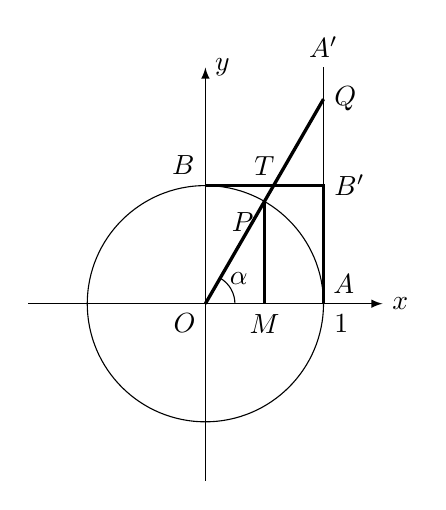
\begin{tikzpicture}[>=latex,scale=1.5]
\draw[->](-1.5,0)--(1.5,0)node[right]{$x$};
\draw[->](0,-1.5)--(0,2)node[right]{$y$};    

\draw(0,0)node[below left]{$O$} circle (1);
\draw(1,0)node[above right]{$A$}--(1,2)node[above]{$A'$};
\draw[very thick](0,0)--(60:1)node[below left]{$P$}--(60:2)node[right]{$Q$};
\draw[very thick](60:1)--(0.5,0)node[below]{$M$};
\draw[very thick](0,1)node[above left]{$B$}--(1,1)node[right]{$B'$}--(1,0)node[below right]{1};
\node at (.5,1)[above]{$T$};
\draw (.25,0) arc (0:60:.25)node[right]{$\alpha$};
\end{tikzpicture}
    \caption{}
\end{figure}


画单位圆$\odot O$(图6.7), 通过单位圆的圆心$O$作互相
垂直的两条直线,其中一条是
水平的,另一条是铅直的,以
$O$为原点,单位圆的半径为长
度单位,在两条直线上建立数
轴,其中水平轴向右为正,铅
直轴向上为正;水平轴用$x$表
示,又叫做$x$轴,铅直的轴用
$y$表示,又叫做$y$轴。以$O$为
顶点,$x$轴的正方向为一边,作$\angle AOP$等于已知角$\alpha$, $\angle AOP$
的两边分别与单位圆相交于$A$、$P$两点,过$P$点作$\overline{PM}\bot OA$于$M$点,

$\because\quad \overline{OP}=1$

$\therefore\quad \sin\alpha=\frac{\overline{MP}}{\overline{OP}}=\overline{MP}\text{的量数},\quad \cos\alpha=\frac{\overline{OM}}{\overline{OP}}=\overline{OM}\text{的量数}$

这样,对于任一锐角$\alpha$, 我们可直接用$\overline{MP}$和$\overline{OM}$的量
数来分别表示$\sin\alpha$, $\cos\alpha$的值。我们把$\overline{MP}$和$\overline{OM}$分别叫做
角$\alpha$的\textbf{正弦线}和\textbf{余弦线}。下面我们用正弦线和余弦线来研究
$\sin\alpha$与$\cos\alpha$的变化规律。

\begin{itemize}
\item 当$\alpha=0^{\circ}$时,$\overline{MP}=0$, 
$\overline{OM}=1$
\item 当$\alpha=90^{\circ}$时,$\overline{MP}=1$, 
$\overline{OM}=0$
\end{itemize}
我们就说,
\[\sin0^{\circ}=0,\qquad
\cos0^{\circ}=1,\qquad
\sin90^{\circ}=1,\qquad
\cos90^{\circ}=0.\]
我们使角$\alpha$从$0^{\circ}$逐渐增加到$90^{\circ}$, 于是从角$\alpha$的正弦线
和余弦线的变化规律可以看到,\textbf{当
$\alpha$增大时,$\sin\alpha$随着增
大,而$\cos\alpha$随着减小;反之,当$\alpha$减小时,$\sin\alpha$随着减小,
而$\cos\alpha$随着增大。}

在图6.7中,过$A$点作$AA'\bot OA$, 与角$\alpha$的一边$OP$相
交于$Q$点,于是,
\[\tan\alpha=\frac{\overline{AQ}}{\overline{OA}}=\overline{AQ}\text{的量数}\]
$\overline{AQ}$叫做角$\alpha$的\textbf{正切线}。

在图6.7中,过单位圆与$y$轴的交点$B$作$BB'\bot OB$, 角
$\alpha$的一边$OP$与$BB'$相交于$T$点,于是,
\[\cot\alpha=\frac{\overline{BT}}{\overline{OB}}=\overline{BT}\text{的量数}\]
$\overline{BT}$叫做角$\alpha$的\textbf{余切线}。

下面我们用正切线和余切线来说明角$\alpha$的正切和余切
随着角$\alpha$的变化规律。

\begin{itemize}
    \item 当$\alpha =0^{\circ}$时,$\overline{AQ}=0$, 边$OP$与$BB'$不相交,我们就说$\tan0^{\circ}=0$,
    $\cot 0^{\circ}$不存在。
    \item 当$\alpha =90^{\circ}$时,$AQ$与$OP$不相交,$\overline{BT}=0$, 
    我们就说,
    $\tan90^{\circ}$不存在,
    $\cot 90^{\circ}=0$.
\end{itemize}

我们使角$\alpha$从$0^{\circ}$增加到$90^{\circ}$, 于是从角$\alpha$的正切线和余
切线的变化规律可以看到,\textbf{当$\alpha$增大时,$\tan\alpha$也随着增大,
而$\cot\alpha$测随着减小。反之当$\alpha$减小时,$\tan\alpha$也随着减小,
而$\cot\alpha$则随着增大。}


\begin{ex}
\begin{enumerate}
    \item 在横线上填入不等号($\alpha$、$\beta$都是锐角)。
    \begin{enumerate}
    \item 当$\alpha>\beta$时,$\sin\alpha\underline{\quad}\sin\beta$,$\cos\alpha\underline{\quad}\cos\beta$,
    $\tan\alpha\underline{\quad}\tan\beta$,$\cot\alpha\underline{\quad}\cot\beta$.
    \item 当$\alpha<\beta$时,$\sin\alpha\underline{\quad}\sin\beta$,$\cos\alpha\underline{\quad}\cos\beta$,
    $\tan\alpha\underline{\quad}\tan\beta$,$\cot\alpha\underline{\quad}\cot\beta$.
    \end{enumerate}

    \item 指出下列差的符号:
\begin{multicols}{2}
\begin{enumerate}
    \item $\sin34^{\circ}-\sin33^{\circ}$
    \item $ \sin27^{\circ}-\sin26^{\circ}$
    \item $\cos83^{\circ}-\cos84^{\circ}$
    \item $\cos10^{\circ}-\cos9^{\circ}$
    \item $\tan 5^{\circ}-\tan 6^{\circ}$
    \item $\cot 14^{\circ}-\cot 13^{\circ}$
    \item $\tan 46^{\circ}-\tan 44^{\circ}$
    \item $\cot 44^{\circ}-\cot 47^{\circ}$
\end{enumerate}
\end{multicols}
\end{enumerate}
\end{ex}

\subsection{$30^{\circ}$、$45^{\circ}$、$60^{\circ}$角的三角比}
我们根据锐角三角比的定义和直角三角形中的一些边角
特殊关系,可以计算出$30^{\circ}$、$45^{\circ}$、$60^{\circ}$角的三角比的精确
值。

作$\triangle ABC$, 使$\angle C=90^{\circ}$,
$\angle A=30^{\circ}$ (图6.8), 那么
$\angle B=60^{\circ}$, 设$\overline{BC}=a$, 则$\overline{AB}=2a$, $\overline{AC}=\sqrt{\overline{AB}^2-\overline{BC}^2}=
\sqrt{(2a)^2-a^2}=\sqrt{3}a$. 
由此得:
\[\begin{split}
    \sin 30^{\circ}=\frac{a}{2a}=\frac{1}{2},&\qquad \sin 60^{\circ}=\frac{\sqrt{3}a}{2a}=\frac{\sqrt{3}}{2}\\
    \cos 30^{\circ}=\frac{\sqrt{3}a}{2a}=\frac{\sqrt{3}}{2},&\qquad \cos 60^{\circ}=\frac{a}{2a}=\frac{1}{2}\\  
\end{split}\]
\[\begin{split}
    \tan 30^{\circ}=\frac{a}{\sqrt{3}a}=\frac{1}{\sqrt{3}}=\frac{\sqrt{3}}{3},&\qquad \tan 60^{\circ}=\frac{\sqrt{3}a}{a}=\sqrt{3}\\
    \cot 30^{\circ}=\frac{\sqrt{3}a}{a}=\sqrt{3},&\qquad \cot 60^{\circ}=\frac{a}{\sqrt{3}a}=\frac{1}{\sqrt{3}}=\frac{\sqrt{3}}{3}\\  
\end{split}\]

\begin{figure}[htp]\centering
    \begin{minipage}[t]{0.48\textwidth}
    \centering
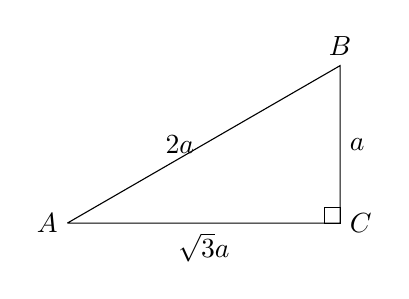
\begin{tikzpicture}[>=latex, scale=1]
     \draw(0,0)node[left]{$A$}--node[below]{$\sqrt{3}a$}(2*1.732,0)node[right]{$C$}--node[right]{$a$}(2*1.732,2)node[above]{$B$}--node[left]{$2a$}(0,0);  
     \draw(2*1.732,0)rectangle (2*1.732-.2,.2);
    \end{tikzpicture}
    \caption{}
    \end{minipage}
    \begin{minipage}[t]{0.48\textwidth}
    \centering
    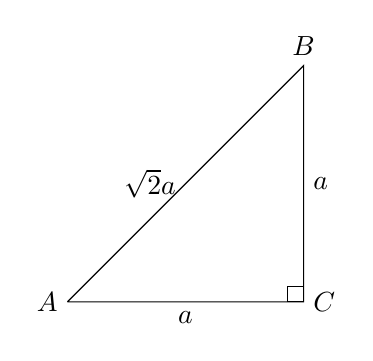
\begin{tikzpicture}[>=latex, scale=1]
 \draw(0,0)node[left]{$A$}--node[below]{$a$}(3,0)node[right]{$C$}--node[right]{$a$}(3,3)node[above]{$B$}--node[left]{$\sqrt{2}a$}(0,0);     
 \draw(3,0)rectangle (3-.2,.2);
    \end{tikzpicture}
    \caption{}
    \end{minipage}
    \end{figure}

作$\triangle ABC$, 使$\angle C=90^{\circ}$, $\angle A=45^{\circ}$ (图6.9), 那么,
$\angle B=45^{\circ}$, 设$\overline{BC}=a$, 则$\overline{AC}=a$, $\overline{AB}=\sqrt{a^2+a^2}=\sqrt{2}a$

由此得:
\[\sin 45^{\circ}=\frac{a}{\sqrt{2}a}=\frac{1}{\sqrt{2}}=\frac{\sqrt{2}}{2},\qquad \cos 45^{\circ}=\frac{a}{\sqrt{2}a}=\frac{1}{\sqrt{2}}=\frac{\sqrt{2}}{2}\]
\[\tan 45^{\circ}=\frac{a}{a}=1,\qquad \cot 45^{\circ}=\frac{a}{a}=1\]
为了便于记忆,我们把$30^{\circ},45^{\circ},60^{\circ}$的三角比列成表。
\begin{center}
    \begin{tabular}{c|ccc}
        \hline
$\alpha$&$30^{\circ}$&$45^{\circ}$&$60^{\circ}$\\
\hline
$\sin\alpha$  &  $\frac{1}{2}$ & $\frac{\sqrt{2}}{2}$& $\frac{\sqrt{3}}{2}$\\
$\cos\alpha$  &  $\frac{\sqrt{3}}{2}$ & $\frac{\sqrt{2}}{2}$& $\frac{1}{2}$\\
$\tan\alpha$  &  $\frac{\sqrt{3}}{3}$ &1&$\sqrt{3}$\\
$\cot\alpha$  &  $\sqrt{3}$ &1&$\frac{\sqrt{3}}{3}$\\
\hline
    \end{tabular}
\end{center}

\begin{example}
    计算 $4\cot 30^{\circ}-2\sin60^{\circ}+2\cos60^{\circ}$
\end{example}

\begin{solution}
\[4\cot 30^{\circ}-2\sin60^{\circ}+2\cos60^{\circ} =4\x \sqrt{3}-2\x \frac{\sqrt{3}}{2}+2\x \frac{1}{2}=3\sqrt{3}+1
\]
\end{solution}


\begin{example}
    计算
$\cos^2 30^{\circ}+\sin^2 45^{\circ}-\tan^2 45^{\circ}$
其中:$\sin^\alpha$、$\cos^2\alpha$
$\tan^2\alpha$、$\cot^2\alpha$分别表示$(\sin\alpha)^2$、$(\cos \alpha)^2$、$(\tan\alpha)^2$、$(\cot \alpha)^2$
\end{example}


\begin{solution}
\[\cos^2 30^{\circ}+\sin^2 45^{\circ}-\tan^2 45^{\circ}=\left(\frac{\sqrt{3}}{2}\right)^2+\left(\frac{\sqrt{2}}{2}\right)^2-1^2=\frac{3}{4}+\frac{2}{4}-1=\frac{1}{4}\]
\end{solution}

\begin{ex}
    求下列各式之值:
\begin{enumerate}
\item $\sin^2 60^{\circ}+\cos^2 30^{\circ}$
\item $\sin^2 60^{\circ}+\cos^2 60^{\circ}$
\item $\sin^2 45^{\circ}+\cos^2 45^{\circ}$
\item $2\sin30^{\circ}+2\cos60^{\circ}+4\tan 45^{\circ}$
\item $5\tan 30^{\circ}+\cot 45^{\circ}-2\tan 45^{\circ}+2\cos 60^{\circ}$  
\item $\frac{2\sin30^{\circ}}{2\cos30^{\circ}-1}$
\item $\frac{\sin60^{\circ}-\sin30^{\circ}}{\sin60^{\circ}+\sin30^{\circ}}$
\end{enumerate}
\end{ex}

\subsection{三角比值表}
在前面的内容中,我们讲的只是特殊角的三角比,为了应用方
便,人们早已制定了任意锐角的三角比值表,下面就来介绍
四位三角比值表的用法。

\subsubsection{正弦表,余弦表}
在正弦、余弦表里左右各有一列排度数,左列上端和右
列下端都有$A$字,在左列$A$的下面,由上到下排着度数,
在右列$A$的上面,由下到上排着度数,在顶行$A$的右边,
由左至右依次排着$0',6',\ldots,60'$, 在表的顶上写着正弦表,
说明查正弦时用左列$A$下面的度数和顶行的分数,表的底下
写着余弦表,说明查余弦时,用右列$A$上的度数和底行的分
数。例如要查$26^{\circ}18'$的正弦,在表中左列$A$的下面先找到
$26^{\circ}$, 顺着$26^{\circ}$所在的这一行往右,在顶行$18'$所在的这一列
里找到了一个数0.4431, 就是$26^{\circ}18'$的正弦,即$\sin26^{\circ}18'=
0.4431$. 换句话说左列$A$下面的$26^{\circ}$所在的行和顶行$18'$所
在的列的交点处的0.4431, 就是$\sin26^{\circ}18'$. 要查$\cos27^{\circ}24'$, 
在表中右列$A$的上面找到$27^{\circ}$, 底行里找到$24'$, $27^{\circ}$所在的
行和$24'$所在的列的交点处的0.8878, 就是$\cos27^{\circ}24'$, 即
$\cos27^{\circ}24'=0.8878$.

\subsubsection{正切表、余切表}
正切的查法和正弦相同,余切的查法和余弦相同,例如
我们在正切表、余切表中可以查到:
\[\tan 54^{\circ}30'=1.4019,\qquad \cot 4^{\circ}6'=13.95\]

\begin{ex}
    查表求下列各三角比:
\begin{enumerate}
    \item $\sin14^{\circ},\quad \sin20^{\circ}24',\quad \sin65^{\circ}30',\quad \sin82^{\circ}12'$
    \item $\cos7^{\circ},\quad  \cos32^{\circ}6',\quad  \cos60^{\circ}54',\quad \cos83^{\circ}18'$
    \item $\tan 18^{\circ},\quad  \tan 78^{\circ}36',\quad  \tan 80^{\circ}24',\quad  \tan 83^{\circ}$
    \item $\cot 42^{\circ}42',\quad   \cot20^{\circ}48', \quad  \cot9^{\circ}36', \quad  \cot 5^{\circ}30'$
\end{enumerate}
\end{ex}

在三角比值表中,最右边的三列是修正值,它是用来求
在左边表里找不到的角的三角比,这三列的上端和下端都标
有$1'$、$2'$、$3'$, 三列中的数是小数的简写,每一个数都代表
一个小数,它的末位数相当于表中间同一行小数的末位数,
$1'$、$2'$、$3'$各列中的各数,分别是它所在的行的角度分别相
差$1'$、$2'$、$3'$时的三角比的修正值,下面举列说明查法:

例如,要求$\sin20^{\circ}19'$, 先从表中查得$\sin20^{\circ}18'$的值是
0.3469, 因为$20^{\circ}19'$比$20^{\circ}18'$大$1'$, 查修正值是0.0003. 因
为角度大,它的正弦值也大,所以$\sin20^{\circ}19'$就比$\sin20^{\circ}18'$
大0.0003, 因此,$\sin20^{\circ}19'=0.3469+0.0003=0.3472$. 要
求$\sin20^{\circ}46'$, 先从表中查得$\sin20^{\circ}48'$的值是0.3551, $20^{\circ}46'$
比$20^{\circ}48'$小$2'$, 查得$2'$的修正值是0.0005, 角度小,正弦值
也小,所以$\sin20^{\circ}46'=0.3551-0.0005=0.3546$. 要求
$\cos28^{\circ}26'$, 先从表中查得$\cos28^{\circ}24'=0.8796$, $28^{\circ}26'$比
$28^{\circ}24'$大$2'$, 查表得修正值是0.0003, 角大余弦值反而小,
所以$\cos28^{\circ}26'=0.8796-0.0003=0.8793$. 

正切的查法和正弦相同,余切的查法和余弦相同。

例如,我们可以求得
\[\tan 69^{\circ}25'=2.662,\qquad \cot 70^{\circ}45'=0.3492\]

\begin{ex}
    查表求下列各三角函数:
\begin{multicols}{2}
    \begin{enumerate}
        \item $\sin18^{\circ}19',\quad  \sin63^{\circ}40'$
        \item $\cos65^{\circ}2',\quad  \cos10^{\circ}34'$
        \item $\tan 9^{\circ}19',\quad  \tan64^{\circ}10'$
        \item $\cot25^{\circ}28',\quad  \cot10^{\circ}25'$
    \end{enumerate}
\end{multicols}
\end{ex}

从三角比值表里不但可以查得任何锐角的三角比,反过
来,也可以根据已知的三角比值查到未知的锐角。

\begin{example}
    已知$\sin x=0.9966$, 求锐角
    $x$.
\end{example}

\begin{solution}
    在正弦表里找到0.9966, 因为它是正弦的值,要用到左
    列的度和顶行的分,在0.9966这一行的左端是$85^{\circ}$, 在0.5966
    的上端是$18'$. 所以
   $ \sin85^{\circ}18'=0.9966$, 因此$x=85^{\circ}18'$.
\end{solution}

\begin{example}
已知$\cos y=0.9966$, 求锐角$y$.
\end{example}

\begin{solution}   
    在表中找到0.9966, 因为它是余弦的值,余弦要用到右
    列的度数和底行的分,在0.9966这一行的右端是$4^{\circ}$, 在
    0.9966这一列的下端是$42'$.

    所以$\cos4^{\circ}42'=0.9966$, 因此$y=4^{\circ}42'$.
\end{solution}

\begin{example}
   $\tan x=14.30$, $\cot y=1.4715$, 求$x$、$y$. 
\end{example}

\begin{solution}
    倒查正切表(查法和例6.6相同)可得:$x=86^{\circ}$.

倒查余切表(查法和例6.7相同)可得:$y=34^{\circ}12'$.
\end{solution}

由三角比值求角度,有时要用到修正值,用修正值时,
必须注意到,对于正弦、正切的值越大,角度也越大;对于
余弦、余切的值越大,角度反而越小,下面举例说明用修正
值查法。

\begin{example}
      $\sin x=0.2493$, 求$x$.
\end{example}

\begin{solution}
在正弦表里,和0.2493最接近的正弦值是0.2487, 它是
$14^{\circ}24'$的正弦,$0.2493-0.2487=0.0006$, 在$14^{\circ}$这一行里
正弦值相差0.0006时,角度的修正值是$2'$, $\sin x$比$\sin14^{\circ}24'$
大0.0006, $x$就比$14^{\circ}24'$大$2'$, 因此
\[x=14^{\circ}24'+2'=14^{\circ}26'\]
\end{solution}

\begin{example}
    $\cos y=0.9841$, 求$y$.
\end{example}

\begin{solution}
    在余弦表中和0.9841最接近的余弦值是0.9842, 它是
$10^{\circ}12'$的余弦,$0.9842-0.9841=0.0001$, 在$10^{\circ}$这一行里
余弦值相差0.0001时,角度的修正值是$1'$或$2'$, $\cos y$比
$\cos10^{\circ}12'$小0.0001, $y$比$12^{\circ}12'$大$1'$或$2'$, 因此
\[y=10^{\circ}12'+1'=10^{\circ}13'\]
或\[y=10^{\circ}12'+2'=10^{\circ}14'\]
这里$y$有两个答案,
一个是不足近似值,一个过剩近似值。
\end{solution}

\begin{example}
    $\tan x=1.3773$, $\cot=0.1950$, 求$x$、$y$.
\end{example}

\begin{solution}
倒查正切表,得$x=54^{\circ}1'$(查法和例6.9相同)。

倒查余切表,得$y=78^{\circ}51'$(查法和例6.10相同)。
\end{solution}

\begin{ex}
    由三角比值表求锐角$x$:
\begin{enumerate}
    \item $\sin x=0.9816,\quad
    \sin x=0.6639,\quad
    \tan x=9.595,\quad
    \tan x=0.1890$
    \item $\cos x=0.8607,\quad
    \cos x=0.9893,\quad
    \cot x=2.106,\quad
    \cot x=67.40$
    \item $\sin x=0.2476,\quad
    \sin x=0.9709,\quad
    \cos x=0.3372$
    
    $
    \cos x=0.4174,\quad
    \tan x=0.365,\quad
    \cot x=0.1614$
\end{enumerate}
\end{ex}

\subsection{互为余角的三角比间的关系}
\begin{figure}[htp]
    \centering
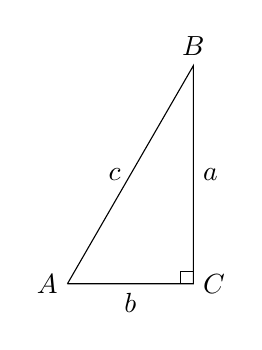
\begin{tikzpicture}[>=latex, scale=.8]
     \draw(0,0)node[left]{$A$}--node[below]{$b$}(2,0)node[right]{$C$}--node[right]{$a$}(2,2*1.732)node[above]{$B$}--node[left]{$c$}(0,0);  
     \draw(2,0)rectangle (2-.2,.2);
    \end{tikzpicture}
    \caption{}
\end{figure}

在直角$\triangle ABC$中,如果$\angle C=90^{\circ}$(图6.10), 则
\[\angle A+\angle B=90^{\circ},\qquad \angle B=90^{\circ}-\angle A\]
由于$\angle A$的对边是$\angle B$的邻边,
$\angle B$的对边是$\angle A$的邻边,那么,根
据三角比的定义,我们便得出$\angle A$和
$\angle B$这两个互为余角的三角比之间有
下面的关系:
\[\begin{split}
    \sin A=\frac{a}{c}=\cos B=\cos(90^{\circ}-A),&\qquad \cos A=\frac{b}{c}=\sin B=\sin(90^{\circ}-A)\\
    \tan A=\frac{a}{b}=\cot B=\cot(90^{\circ}-A),&\qquad \cot A=\frac{b}{a}=\tan B=\tan(90^{\circ}-A)\\
\end{split}\]

这就是说,\textbf{互为余角的两个角中,任一角的正弦等于另
一角的余弦;任一角的正切等于另一角的余切。}

有了这个关系,我们就可把任意大于$45^{\circ}$的锐角的三角
比化为小于$45^{\circ}$的锐角的三角比。

\begin{example}
    把下面各角的三角比化为小于$45^{\circ}$的锐角的三角
    比。
\begin{multicols}{2}
\begin{enumerate}
\item $\sin75^{\circ}$
\item $\cos62^{\circ}22'$
\item $\tan 80^{\circ}$
\item $\cot56^{\circ}18'$
\end{enumerate}
\end{multicols}
\end{example}

\begin{solution}
\begin{enumerate}
    \item $\sin75^{\circ}=\cos(90^{\circ}-75^{\circ})=\cos 15^{\circ}$
    \item $\cos62^{\circ}22'=\sin(90^{\circ}-62^{\circ}22')=\sin27^{\circ}38'$
    \item $\tan 80^{\circ}=\cot(90^{\circ}-80^{\circ})=\cot10^{\circ}$
    \item $\cot 56^{\circ}18'=\tan(90^{\circ}-56^{\circ}18')=\tan 33^{\circ}42'$
\end{enumerate}
\end{solution}


\begin{example}
    下列等式是否成立:
\begin{enumerate}
\item $\sin(60^{\circ}+\alpha )=\cos(30^{\circ}-\alpha ) \qquad (0\le \alpha \le 30^{\circ})$
\item $\sin(45^{\circ}+\alpha )=\cos(45^{\circ}-\alpha ) \qquad (0\le \alpha \le 45^{\circ})$
\item $\tan(50^{\circ}+\alpha )=\cot (40^{\circ}-\alpha ) \qquad (0\le \alpha <40^{\circ})$
\end{enumerate}
\end{example}


\begin{solution}
由于
\[\begin{split}
    (60^{\circ}+\alpha )+(30^{\circ}-\alpha )&=90^{\circ}\\
(45^{\circ}+\alpha )+(45^{\circ}-\alpha )&=90^{\circ}\\
(50^{\circ}+\alpha )+(40^{\circ}-\alpha )&=90^{\circ}
\end{split}\]

而$\alpha $角的取值范围使得各式中的三角比都有意义,所以
根据互为余角的三角比之间的关系可知,各等式都成立。
\end{solution}

\begin{ex}
    \begin{enumerate}
        \item 为什么三角比值表中,锐角$\alpha$的正弦和$90^{\circ}-\alpha$角的余弦共
        用一个表。
\item 把下列各角的三角比化为小于$45^{\circ}$的锐角的三角比。
\begin{multicols}{2}
\begin{enumerate}
    \item $\sin73^{\circ},\qquad \sin77^{\circ}18'$
    \item $\cos57^{\circ},\qquad \cos52^{\circ}38'$
    \item $\tan78^{\circ},\qquad \tan79^{\circ}5'$
    \item $\cot48^{\circ},\qquad \cot78^{\circ}31'$
\end{enumerate}
\end{multicols}
\item 下列各式中的$x$应为多少度?
\begin{multicols}{2}
\begin{enumerate}
    \item $\sin75^{\circ}=\cos x$
    \item $\cos18^{\circ}=\sin x$
    \item $\tan5^{\circ}=\cot x$
    \item $\cot83^{\circ}=\tan x$
\end{enumerate}
\end{multicols}
\item 下列等式是否成立($x$、$\alpha$的取值都使各三角比有意义)。
\begin{multicols}{2}
\begin{enumerate}
    \item $\sin(75^{\circ}+\alpha )=\cos(15^{\circ}-\alpha )$
    \item $\sin(15^{\circ}-\alpha )=\sin(30^{\circ}+\alpha )$
    \item $ \tan (30^{\circ}+x)=\cot (60^{\circ}-x)$
    \item $ \cot (89^{\circ}+\alpha )=\tan (1^{\circ}-\alpha )$
\end{enumerate}
\end{multicols}
    \end{enumerate}
\end{ex}

\subsection{同一锐角的各三角比间的关系}
\begin{blk}{定理}
    同一锐角$\alpha$ 的四个三角比之间有下列关系:
\begin{enumerate}
    \item $\sin^2\alpha  +\cos^2\alpha =1$
    \item $\tan\alpha=\frac{\sin\alpha}{\cos\alpha },\qquad \cot\alpha=\frac{\cos\alpha }{\sin\alpha }$
    \item $\tan\alpha\cdot \cot\alpha =1$
\end{enumerate}
\end{blk}

\begin{proof}
    作直角$\triangle ABC$, 使$\angle C=90^{\circ}$, $\angle A=\alpha$ (图6.11).
    \begin{figure}[htp]
        \centering
    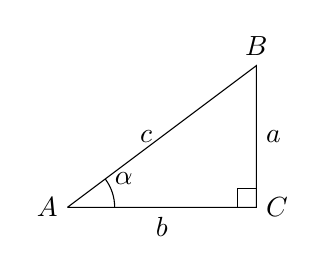
\begin{tikzpicture}[>=latex, scale=1.2]
         \draw(0,0)node[left]{$A$}--node[below]{$b$}(2,0)node[right]{$C$}--node[right]{$a$}(2,1.5)node[above]{$B$}--node[left]{$c$}(0,0);  
         \draw(2,0)rectangle (2-.2,.2);
         \draw (.5,0) arc (0:36.87:.5)node[right]{$\alpha$};
        \end{tikzpicture}
        \caption{}
    \end{figure}
    
\begin{enumerate}
    \item $\because\quad  a^2+b^2=c^2$
    
    $\therefore\quad \left(\frac{a}{c}\right)^2+\left(\frac{b}{c}\right)^2=1$

    又$\because\quad \frac{a}{c}=\sin\alpha,\quad \frac{b}{c}=\cos\alpha$,

    $\therefore\quad \sin^2\alpha  +\cos^2\alpha =1$,即:
\textbf{一锐角的正弦和余弦的平方和等于1.}
该式也就是勾股定理的三角比的表示式。

\item $\because\quad \tan\alpha=\frac{a}{b},\quad \frac{\sin\alpha}{\cos\alpha}=\frac{\frac{a}{c}}{\frac{b}{c}}=\frac{a}{b}$,

$\therefore\quad \tan\alpha=\frac{\sin\alpha}{\cos\alpha}$

又$\because\quad \cot\alpha=\frac{b}{a},\quad \frac{\cos\alpha}{\sin\alpha}=\frac{\frac{b}{c}}{\frac{a}{c}}=\frac{b}{a}$,

$\therefore\quad \cot\alpha=\frac{\cos\alpha}{\sin\alpha}$

\item $\because\quad \tan\alpha=\frac{a}{b},\quad \cot\alpha=\frac{b}{a}$

$\therefore\quad \tan\alpha\cdot \cot\alpha=\frac{a}{b}\cdot \frac{b}{a}=1$
\end{enumerate}
\end{proof}

上面的定理,表示了同一锐角的三角比之间的关系,我
们可利用定理中的三个公式,由已知锐角的一个三角比,去
计算这个角的其它的三个三角比;也可以利用它们来化简含
有三角比的式子。


\begin{example}
    已知:$\sin\alpha=\frac{3}{5}$, 
    求$\alpha$角($\alpha$为锐角)的其它
    的三个三角比。
\end{example}


\begin{solution}
 从公式$\sin^2\alpha +\cos^2\alpha =1$ 可得
   \[ \cos\alpha =\pm\sqrt{1-\sin^2\alpha}\] 
   由于锐角的三角比都是正
    数,所以根号前应取正号,把$\sin\alpha =\frac{3}{5}$
    代入上式,得
\[\cos\alpha=\sqrt{1-\left(\frac{3}{5}\right)^2}=\sqrt{\frac{25-9}{5^2}}=\frac{4}{5}\]
根据$\tan\alpha=\frac{\sin\alpha}{\cos\alpha}$,可得
\[\tan\alpha=\frac{\frac{3}{5}}{\frac{4}{5}}=\frac{3}{4}\]
再根据$\tan\alpha\cdot \cot\alpha=1$,可得
\[\cot\alpha=\frac{4}{3}\]
\end{solution}

\begin{example}
    化简
    $\sin^2 54^{\circ}+\sin^2 36^{\circ}-\tan 45^{\circ}$
\end{example}

\begin{solution}
\[\begin{split}
    \sin^2 54^{\circ}+\sin^2 36^{\circ}-\tan 45^{\circ}&=
    \cos^2(90^{\circ}-54^{\circ})+\sin^2 36^{\circ}-\tan 45^{\circ}\\
    &=\cos^2 36^{\circ}+\sin^2 36^{\circ}-1\\
    &=1-1=0
\end{split}\]
\end{solution}


\begin{example}
    化简$\frac{\sqrt{1-\sin^2\alpha}}{\sin\alpha}\cdot \tan\alpha$
\end{example}

\begin{solution}
    \[\frac{\sqrt{1-\sin^2\alpha}}{\sin\alpha}\cdot \tan\alpha=\frac{\cos\alpha}{\sin\alpha}\cdot \tan\alpha=\cot\alpha\cdot \tan\alpha=1\]
\end{solution}

\begin{example}
    化简$(\sin\alpha+\cos\alpha)^2+(\sin\alpha-\cos\alpha)^2$
\end{example}

\begin{solution}
\[\begin{split}
&    (\sin\alpha+\cos\alpha)^2+(\sin\alpha-\cos\alpha)^2\\  
&\quad =\sin^2\alpha+2\sin\alpha\cdot \cos\alpha+\cos^2\alpha
+\sin^2\alpha-2\sin\alpha\cdot\cos\alpha+\cos^2\alpha\\
&\quad =1+1=2
\end{split}\]    
\end{solution}

\begin{ex}
\begin{enumerate}
    \item 证明$\sin^2\alpha+\cos^2\alpha=1$, $\tan\alpha=\frac{\sin\alpha}{\cos\alpha}$
    \item 已知$\sin\alpha=\frac{5}{13}$,求$\cos\alpha, \tan\alpha, \cot\alpha$
    \item 已知$\cos\alpha=\frac{4}{5}$,求$\sin\alpha, \tan\alpha, \cot\alpha$
    \item 已知$\tan\alpha=\frac{3}{4}$,求$\sin\alpha,\cos\alpha$。
    
提示:$\tan^2\alpha =\frac{\sin^2\alpha}{1-\sin^2\alpha}=\frac{9}{16}$,令$\sin \alpha =x$,解方程。

\item 化简

\begin{enumerate}\begin{multicols}{2}
    \item $\frac{1-\sin^2\alpha}{\cos^2\alpha}$
    \item $\tan\alpha\cdot \cos\alpha$
    \item $\frac{\cos\alpha}{\sqrt{1-\cos^2\alpha}}$
    \item $\frac{\sin^2\alpha}{1+\cos\alpha}$
    \item $\frac{\cos^2\alpha}{1-\sin\alpha}$\end{multicols}
    \item $(\tan\alpha+\cot\alpha)^2-(\tan\alpha-\cot\alpha)^2$
\end{enumerate}

\end{enumerate}
\end{ex}

\subsection*{习题6.1}
\begin{enumerate}
    \item 在直角$\triangle ABC$中,$\angle C=90^{\circ}$, $a=3$, $b=2$, 求$\angle A$的四
    个三角比。
    \item 在直角$\triangle ABC$中,$\angle C=90^{\circ}$,$\overline{AB}=10$, $\overline{BC}=8$, 求:
   $ \sin A$、$\cos A$.
    \item 在直角$\triangle ABC$中,$\angle C=90^{\circ}$, $\overline{CD}$为$\overline{AB}$边上的高,问
    图中哪些线段的比可以表
    示$\angle A$的正弦?哪些线段
    的比可以表示$\angle B$的正弦?
\begin{figure}[htp]
    \centering
    \begin{tikzpicture}
\draw(0,0)node[below]{$A$}--(5,0)node[below]{$B$}--(3.2,2.4)node[above]{$C$}--(0,0);
\draw(3.2,2.4)--(3.2,0)node[below]{$D$};
\draw(3.2,0) rectangle (3.2+.2,.2);        
\draw (0.4,0) arc (0:32:.4);
\draw (3.2,2) arc (-90:-90+32:.4);
    \end{tikzpicture}
    \caption*{第3题}
\end{figure}

    \item 判断下列等式是否正确:
\begin{enumerate}
\item $\sin35^{\circ} 30'=\cos54^{\circ} 30'$
\item $\sin(30^{\circ} -\alpha )=\cos(60^{\circ} +\alpha )$
\item $\cos(2\alpha +14^{\circ} )=\sin(76^{\circ} -2\alpha )$
\end{enumerate}

\item 化简下列各式:
\begin{enumerate}
\item $\sin^4\alpha  +2\sin^2\alpha \cos^2\alpha +\cos^4\alpha $
\item $\sin^4\alpha -\cos^4\alpha +\cos^2\alpha $
\item $\sin(45^{\circ} +\alpha )-\cos(45^{\circ} -\alpha )$    
\item $\frac{1-\sin^2\alpha }{1-\cos^2\alpha }$
\item $\frac{\tan \alpha +\tan \beta}{\cot\alpha +\cot \beta}$
\item $\sin(90^{\circ} -\alpha )\cdot \cot(90^{\circ} -\alpha )$
\end{enumerate}

\item 已知 $\tan \alpha =2$, 求 $\tan(90^{\circ} -\alpha )$.
\item 已知
$\sin A=\frac{1}{3}$
求 $\cos A$, $\tan A$.
\item 已知互为余角的两角的正切的和等于3, 求两角正切的
平方和。
\item 求下列各题中的未知锐角$x$:
\begin{multicols}{2}
\begin{enumerate}
    \item $\sin x=\frac{1}{2}$
    \item $\cos x=\frac{\sqrt{2}}{2}$
    \item $\tan x=\sqrt{3}$
    \item $\sin x=\frac{\sqrt{3}}{2}$
    \item $\cos x=\frac{1}{2}$
    \item $\tan x=\frac{1}{\sqrt{3}}$
\end{enumerate}
\end{multicols}

\item 已知 $\cos^2 x=\frac{1}{4}$,求$x$.
\item 已知 $\cos^2x-\sin^2x=\frac{1}{2}$, 
求$x$.
\item 回答下列问题:
\begin{enumerate}
\item 当$0^{\circ}\le \alpha\le 90^{\circ}$时,$\sin\alpha$的最大值是多少?最小值
是多少?
\item 当$0^{\circ}\le \alpha\le 90^{\circ}$时,$\cos\alpha$的最大值是多少?最小值
是多少?
\end{enumerate}


\item 当$0^{\circ}\le \alpha\le 45^{\circ}$, $\alpha=45^{\circ}$, $45^{\circ}<\alpha\le 90^{\circ}$时,分别比较
$\sin\alpha$与$\cos\alpha$的大小。
\end{enumerate}

\section{解直角三角形}
\subsection{直角三角形中的边角关系}

我们把学过的直角三角形中
的边角基本关系总结如下:
\begin{figure}[htp]
    \centering
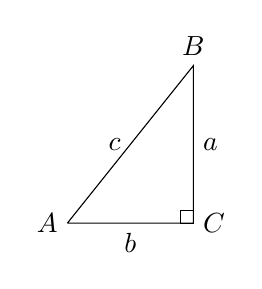
\begin{tikzpicture}[>=latex, scale=.8]
     \draw(0,0)node[left]{$A$}--node[below]{$b$}(2,0)node[right]{$C$}--node[right]{$a$}(2,2.5)node[above]{$B$}--node[left]{$c$}(0,0);  
     \draw(2,0)rectangle (2-.2,.2);
    \end{tikzpicture}
    \caption{}
\end{figure}

已知$\triangle ABC$, $\angle C=90^{\circ}$ (图6.12).
\begin{enumerate}
    \item 勾股定理:$a^2+b^2=c^2$
    \item 两锐角互余:$\angle A+\angle B=90^{\circ}$
    \item 四个三角比:
\[\sin A=\frac{\angle A\text{的对边}}{\angle A\text{斜边}},\qquad \cos A=\frac{\angle A\text{的邻边}}{\angle A\text{斜边}}\]
\[\tan A=\frac{\angle A\text{的对边}}{\angle A\text{的邻边}},\qquad \cot A=\frac{\angle A\text{的邻边}}{\angle A\text{的对边}}\]
\end{enumerate}
    为了应用方便,我们把3中的四个公式写成下面的形
    式:
\[\angle A\text{的对边}=\text{斜边}\x \sin A,\qquad \angle A\text{的邻边}=\text{斜边}\x \cos A\]
\[\angle A\text{的对边}=\text{邻边}\x \tan A,\qquad \angle A\text{的邻边}=\text{对边}\x \cot A\]

改用语言叙述,就是:
\begin{blk}{}
 在直角三角形中:
\begin{enumerate}
\item 一条直角边等于斜边乘上这条直角边所对锐角的
正弦。
\item 一条直角边等于斜边乘上这条直角边相邻锐角的
余弦。
\item 一条直角边等于另一条直角边乘上这条直角边所
对锐角的正切。
\item 一条直角边等于另一条直角边乘上这条直角边相
邻锐角的余切。
\end{enumerate}
\end{blk}

\begin{ex}
    \begin{enumerate}
        \item 在直角$\triangle ABC$中,$\angle C=90^{\circ}$, 求证:
\[\overline{AB}=\frac{\overline{BC}}{\sin A},\qquad \overline{AB}=\frac{\overline{AC}}{\cos A}\]
       并把这两个式子用语言叙述出来。
        \item 在直角$\triangle ABC$中,$\angle C=90^{\circ}$,求证:
\begin{enumerate}
    \item $\sin A=\cos B,\qquad      \sin B=\cos A$
    \item $\tan A=\cot B,\qquad \cot A=\tan B$
\end{enumerate}
    \end{enumerate}

\end{ex}

\subsection{解直角三角形}
根据三角形的某些已知元素求出它的未知元素,这种过
程叫做\textbf{解三角形}。在直角三角形中,直角总是已知的。除直
角外,只要再知道两个元素,其中至少有一边,就可以求出
直角三角形的其它各元素。因此,解直角三角形,只有下面
四种情况:
\begin{enumerate}
    \item 已知斜边与一锐角,
    \item 已知一条直角边与一锐角;
    \item 已知斜边与一条直角边;
    \item 已知两条直角边。
\end{enumerate}

上述四种情况,都可用前面中所列出的关系式,并利用
三角比值表来求解。

\begin{example}
    已知$c=18$, $\angle A=62^{\circ}20'$ (图6.13),
求:$\angle B, a, b$
\end{example}

\begin{solution}
\[\begin{split}
    \angle B&=90^{\circ}-\angle A=90^{\circ}-62^{\circ}20'
=27^{\circ}40'\\
a&=c\sin A=18\x \sin62^{\circ}20'=18\x0.8857
\approx 15.9\\
b&=c\cos A=18\x\cos62^{\circ}20'=18\x0.4643\approx 8.3600
\end{split}\]
\end{solution}

\begin{figure}[htp]\centering
    \begin{minipage}[t]{0.48\textwidth}
    \centering
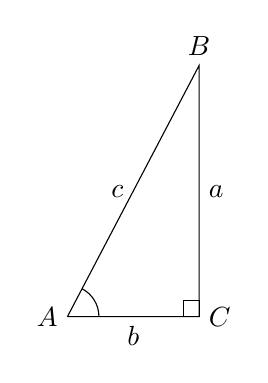
\begin{tikzpicture}[>=latex, scale=2]
    \draw(0,0)node[left]{$A$}--node[below]{$b$}(.8358,0)node[right]{$C$}--node[right]{$a$}(62.33:1.8)node[above]{$B$}--node[left]{$c$}(0,0);  
    \draw(.8358,0)rectangle (.8358-.1,.1);
    \draw(.2,0) arc (0:62.33:.2);
    \end{tikzpicture}
    \caption{}
    \end{minipage}
    \begin{minipage}[t]{0.48\textwidth}
    \centering
    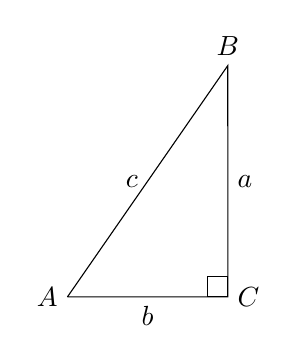
\begin{tikzpicture}[>=latex, scale=1.3]
\draw(0,0)node[left]{$A$}--node[below]{$b$}(1.567,0)node[right]{$C$}--node[right]{$a$}(55.27:2.75)node[above]{$B$}--node[left]{$c$}(0,0);  
    \draw(1.567,0)rectangle (1.567-.2,.2);
    \end{tikzpicture}
    \caption{}
    \end{minipage}
    \end{figure}

\begin{example}
    已知$c=27.5$, $a=22.6$, 求$b$、$\angle A$、$\angle B$ (图6.14).
\end{example}

\begin{solution}
\[b=\sqrt{c^2-a^2}=\sqrt{27.5^2-22.6^2}\approx 15.7\]
由于
$\sin A=\frac{a}{c}=\frac{22.6}{27.5}\approx 0.8218$,
因此:
\[\begin{split}
    \angle A&\approx 55^{\circ}16'\\
\angle B&=90^{\circ}-\angle A=90^{\circ}-55^{\circ}16'=34^{\circ}44'
\end{split}\]
\end{solution}


\begin{example}
    已知$a=3.8$, $\angle A=42^{\circ}$, 求$\angle B$, $C$, $b$ (图6.15).
\end{example}

\begin{solution}
\[\begin{split}
    B&=90^{\circ} -\angle A=48^{\circ} \\
b&=a \cot A=3.8\x\cot 42^{\circ}\approx 4.22\\
c&=\frac{a}{\sin A}=\frac{3.8}{\sin 42^{\circ}}\approx 5.68 
\end{split}\]
    
\end{solution}

\begin{figure}[htp]\centering
    \begin{minipage}[t]{0.48\textwidth}
    \centering
\begin{tikzpicture}[>=latex, scale=.7]
    \draw(0,0)node[left]{$A$}--node[below]{$b$}(4.22,0)node[right]{$C$}--node[right]{$a$}(42:5.68)node[above]{$B$}--node[left]{$c$}(0,0);  
    \draw(4.22,0)rectangle (4.22-.2,.2);
    \draw(.6,0) arc (0:42:.6);
    \end{tikzpicture}
    \caption{}
    \end{minipage}
    \begin{minipage}[t]{0.48\textwidth}
    \centering
    \begin{tikzpicture}[>=latex, scale=.8]
\draw(0,0)node[left]{$B$}--node[below]{$c$}(5,0)node[right]{$A$}--node[right]{$b$}(90-36.87:3)node[above]{$C$}--node[left]{$a$}(0,0);  
  
    \end{tikzpicture}
    \caption{}
    \end{minipage}
    \end{figure}


\begin{example}
    已知$a=3$、$b=4$, 求$c$、$\angle A$、$\angle B$ (图6.16)
\end{example}

\begin{solution}
\[c=\sqrt{a^2+b^2}=\sqrt{3^2+4^2}=5\]
由于$\tan A=\frac{3}{4}=0.75$,
因此:$$\angle A\approx 36^{\circ} 52',\qquad 
\angle B\approx 90^{\circ} -36^{\circ} 52'=53^{\circ} 8'$$ 
\end{solution}

\begin{ex}
\begin{enumerate}
    \item 解下列直角三角形:
    \begin{enumerate}
    \item 已知$c=58.5,\quad \angle A=45^{\circ} 13'$
    \item 已知$c=14,\quad \angle B=62^{\circ}$
    \item 已知$c=28,\quad \angle A=34^{\circ} $
    \item 已知$c=195,\quad \angle B=78^{\circ} 47'$
    \item 已知$a=87,\quad \angle A=55^{\circ} $
    \item 已知$b=99,\quad \angle B=83^{\circ} $
    \item 已知$c=32,\quad a=18$
    \item 已知$a=14,\quad \angle B=78^{\circ}$
    \item 已知$c=79,\quad b=56$
    \item 已知$a=12.8,\quad b=15.6$
    \item 已知$c=73,\quad \angle B=66.2^{\circ}$ 
    \item 已知$c=350,\quad \angle A=3.8^{\circ} $
\end{enumerate}

\item 已知直角$\triangle ABC$, $\angle C=90^{\circ}$, $\angle A=\alpha$和$\angle A$对的直角边是
$a$

求证:直角$\triangle ABC$的面积$S=\frac{a^2}{2}\tan\alpha$

\item  已知直角三角形的一个锐角为$\alpha$, 面积等于$S$, 
求它的外接圆的面积。
\end{enumerate}
\end{ex}

\subsection{解直角三角形的应用}
下面我们举例说明解直角三角形在实际中的应用。






\begin{example}
    
\end{example}

\begin{example}
    
\end{example}


\begin{solution}
    
\end{solution}

\begin{solution}
    
\end{solution}

\begin{solution}
    
\end{solution}
\begin{example}
    
\end{example}

\begin{example}
    
\end{example}

\begin{solution}
    
\end{solution}






\begin{example}
    
\end{example}

\begin{solution}
    
\end{solution}

\begin{example}
    
\end{example}   

    \begin{solution}
    
\end{solution}

\begin{example}
 
    
\end{example}

\begin{solution}
    
\end{solution}

\begin{example}
    
\begin{solution}
    
\end{solution}
    
\end{example}

\begin{solution}
    
\end{solution}


\begin{solution}
    
\end{solution}

\begin{solution}
    
\end{solution}

\begin{solution}
    
\end{solution}

\begin{solution}
    
\end{solution}






